\section{Intra-domain Routing Protocol: IS-IS}
\label{sec:isis}

\subsection{Design}

IS-IS is short for Intermediate System to Intermediate System Routing Protocol. In this lab, the IS-IS is used as the Interior Gateway Protocol (IGP). 
By using this protocol, each router maintains a database which has a map of the whole topology and all routers have the same information. The best path to every destination is computed by all routers. 
Figure \ref{fig:isis} shows the design of IS-IS protocol in BT Network. As the figure shows, the network only has level-1 routers for internal routing.

\begin{figure}[ht!]
    \centering
    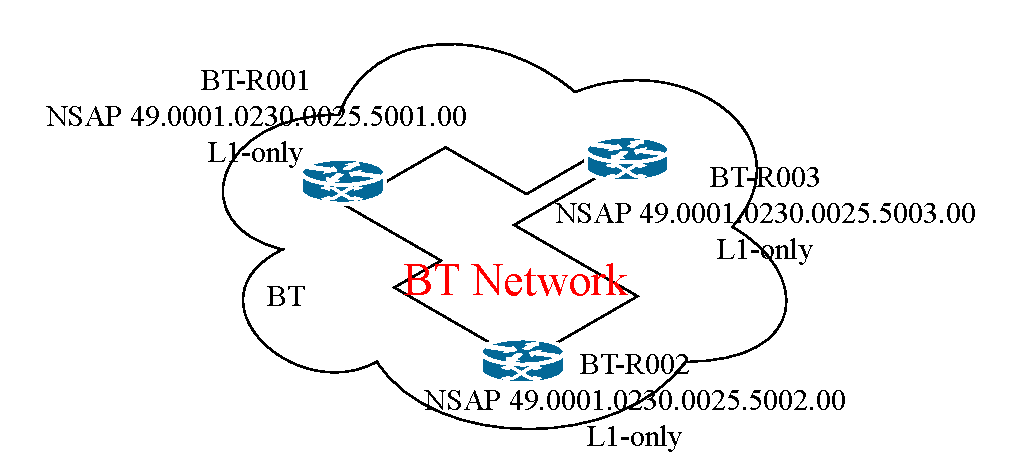
\includegraphics[width=0.8\linewidth]{isis}
    \caption{Design of IS-IS Protocol in BT Network.}
    \label{fig:isis}
\end{figure}

\subsection{Loopback Addresses and NSAP for Routers}

To set up IS-IS, an unique loopback address is needed for each router. 
An IPv4 address block of \texttt{23.0.255.0/24} and IPv6 address block of \texttt{2001:2300:ffff::/48} is allocated for loopback addresses. 

Following the CLNS addressing convention, each router is then assigned with a NSAP. A NSAP has $3$ main components. 

According to the convention, the leading Area ID is composed of AFI ($49$) and Area Address ($0001$). 
The System ID followed is set to the IPv4 loopback address of the router. If the loopback address is $ABC.DEF.GHI.JKL$, then System ID should be $ABCD.EFGH.IJKL$.
The last main component is N-Selector (NSEL) and set to $00$.

The assignment of addresses and NSAP to routers are detailed in Table \ref{tab:isis}.

\begin{longtable}[]{@{}llll@{}}
\toprule
Router & IPv4 Loopback Address & IPv6 Loopback Address & NSAP\tabularnewline
\midrule
\endhead
BT-R001 & 23.0.255.1 & 2001:2300:ffff:1:: & 49.0001.0230.0025.5001.00\tabularnewline
BT-R002 & 23.0.255.2 & 2001:2300:ffff:2:: & 49.0001.0230.0025.5002.00\tabularnewline
BT-R003 & 23.0.255.3 & 2001:2300:ffff:3:: & 49.0001.0230.0025.5003.00\tabularnewline
\bottomrule
\caption{IP Loopback Addresses and NSAP for Routers in BT Network.}
\label{tab:isis}
\end{longtable}



\subsection{Implementation}

IS-IS is set up on Router 1 (BT-R001) using the following commands.

\begin{lstlisting}
interface Loopback0
ip address 23.0.255.1 255.255.255.255
ipv6 address 2001:2300:FFFF:1::/128

router isis
net 49.0001.0230.0025.5001.00
is-type level-1
\end{lstlisting}

Then, IS-IS is turned on on all interfaces to internal routers.

\begin{lstlisting}
interface FastEthernet0/0
ip router isis
ipv6 router isis

interface FastEthernet0/1
ip router isis
ipv6 router isis

interface FastEthernet0/1/0
ip router isis
ipv6 router isis
\end{lstlisting}

\clearpage

However, IS-IS routes should not be broadcasted nor received through the loopback interface (\texttt{Loopback0}) while the route to corresponding subnet should be broadcasted to other internal routers. Therefore, the loopback interface should be a passive interface in IS-IS protocol.

\begin{lstlisting}
router isis
passive-interface Loopback0
\end{lstlisting}

For Router 2 (BT-R002) and Router 3 (BT-R002), IS-IS is set up similarly using the above commands. The main difference is that interfaces to external routers (VLAN 3 for Router 2 and VLAN 4 \& 5 for Router 3) should be passive interfaces as well. Below is the configuration for Router 2.

\begin{lstlisting}
interface Loopback0
ip address 23.0.255.2 255.255.255.255
ipv6 address 2001:2300:FFFF:2::/128

router isis
net 49.0001.0230.0025.5002.00
is-type level-1
passive-interface Vlan3
passive-interface Loopback0

interface FastEthernet0/0
ip router isis
ipv6 router isis

interface FastEthernet0/1
ip router isis
ipv6 router isis

interface Vlan1
ip router isis
ipv6 router isis
\end{lstlisting}

\subsection{Evaluation}

Once the IS-IS is set up, use \texttt{traceroute} command to check the path from Laptop 1 (BT001, IPv4 Address: 23.0.0.2) to Laptop 2 (BT002, IPv4 Address: 23.0.0.18) in the network.

\begin{lstlisting}[language=sh]
traceroute 23.0.0.34
\end{lstlisting}

Figure \ref{fig:isis-traceroute} shows the route taken is 
\texttt{Laptop 1 (BT001, IPv4 Address: 23.0.0.2)
-> Router 1 (BT-R001, IPv4 Address: 23.0.0.1) 
-> Router 2 (BT-R002, IPv4 Address: 23.0.0.50)
-> Laptop 2 (BT002, IPv4 Address: 23.0.0.18)}, which is a correct route.
Routes from Laptop 1 to Laptop 3 as well as from Laptop 2 to Laptop 3 are tested in the figure as well.

\begin{figure}[ht!]
    \centering
    \begin{subfigure}[b]{\textwidth}
        \centering
        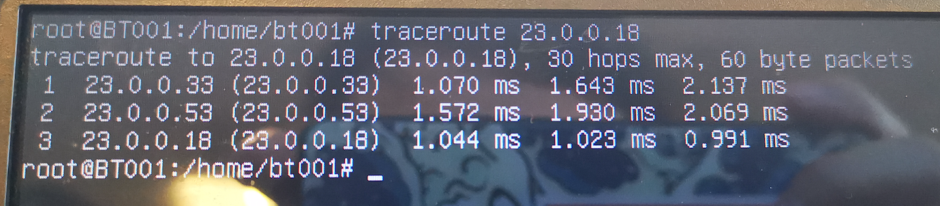
\includegraphics[width=\linewidth]{isis-traceroute-1-2}
        \caption{\texttt{traceroute} from Laptop 1 (BT001) to Laptop 2 (BT002)}
    \end{subfigure}
    ~
    \begin{subfigure}[b]{\textwidth}
        \centering
        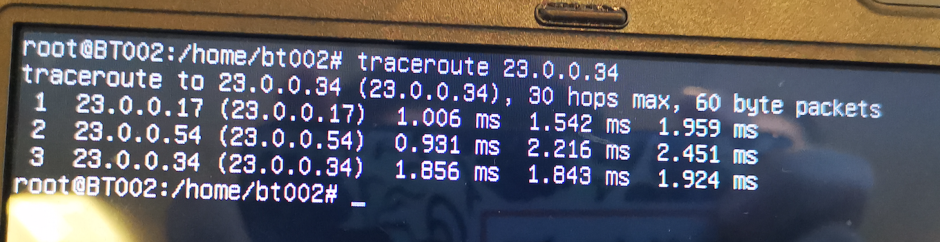
\includegraphics[width=\linewidth]{isis-traceroute-2-3}
        \caption{\texttt{traceroute} from Laptop 2 (BT002) to Laptop 3 (BT003)}
    \end{subfigure}
    \caption{Running \texttt{traceroute} between Laptops in BT Network.}
    \label{fig:isis-traceroute}
\end{figure}

To further evaluate the correctness of our implementation, we check the path from Laptop 1 to Laptop 2 under the condition that the physical connection between Router 1 and Router 2 is broken. The IS-IS protocol on Router 1 should be able to find route to Router 2 through Router 3.

Figure \ref{fig:isis-traceroute-broken} shows the route taken is 
\texttt{Laptop 1 (BT001, IPv4 Address: 23.0.0.2)
-> Router 1 (BT-R001, IPv4 Address: 23.0.0.1) 
-> Router 3 (BT-R003, IPv4 Address: 23.0.0.58) 
-> Router 2 (BT-R002, IPv4 Address: 23.0.0.53)
-> Laptop 2 (BT002, IPv4 Address: 23.0.0.18)}, which is a correct route.


\begin{figure}[ht!]
    \centering
    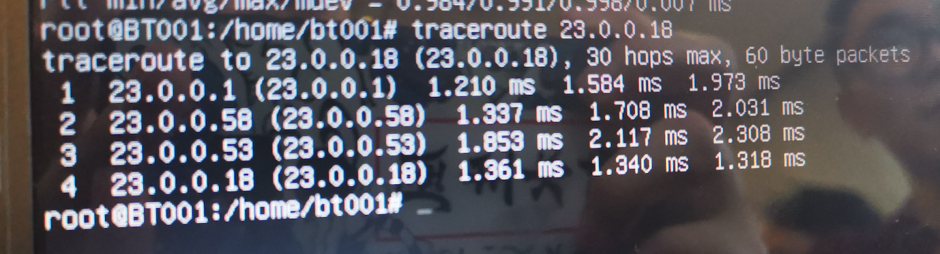
\includegraphics[width=0.8\linewidth]{isis-traceroute-broken-1-2}
    \caption{\texttt{traceroute} from Laptop 2 (BT002) to Laptop 3 (BT003) when Physical Connection between Router 1 (BT-R001) and Router 2 (BT-R002) is broken.}
    \label{fig:isis-traceroute-broken}
\end{figure}


\subsection{Commentary}

\subsubsection{Problem: IS-IS Not Set Up for Laptop-Router Interface}
When initially setting up IS-IS on the interfaces, only the interfaces between routers have been turned on. This leads to laptop's failure to reach a router not directly connected.
To solve this problem, IS-IS is set up on the interface between a laptop and a router.




